\subsection{Overview}
In this section we describe the architectural design of our system, the main components and their interactions. \\
The system will be described starting with high-level components. Then a more detailed description is provided for the client and the database structure, including the architectural patterns applied.

\subsection{High level components}
The main high level components of our system are:
\begin{itemize}
\item {\textbf{Client}}: this component is responsible for the visualization of data (front-end) and for the management of requests and replies to and from the services providing data to the system.
\item {\textbf{Firebase}}: this component is responsible for the storage of the permanent data of the users and for the registration and login of users; we use the services provided by Firebase to manage these data.
\item {\textbf{Marvel APIs}}: we use the APIs provided by Marvel in order to always have complete and up-to-date data on comics.
\item {\textbf{Facebook}}: used for the login procedure.
\item {\textbf{Google}}: used for the login procedure.
\end{itemize}

\vspace{3mm}

\begin{figure}[h]
\centering
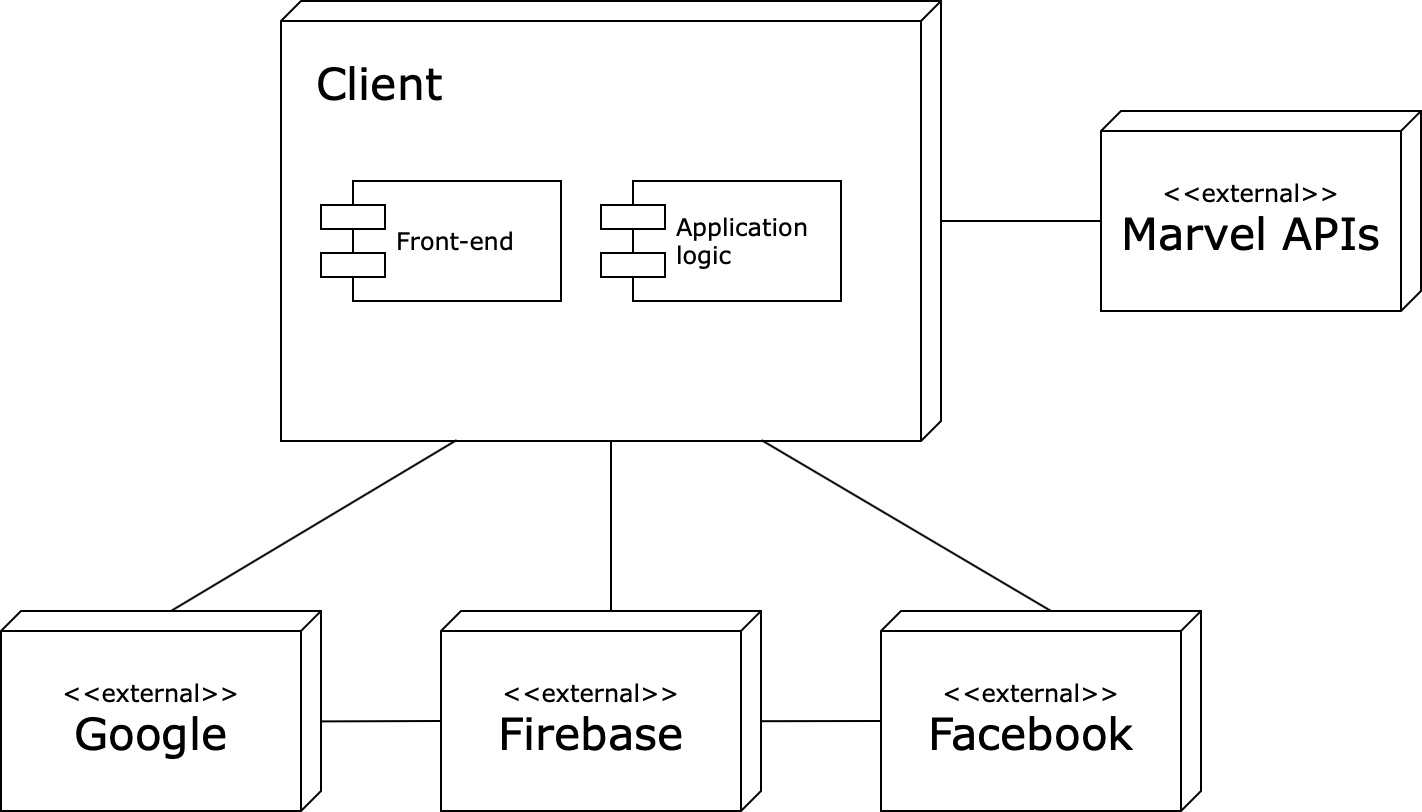
\includegraphics[width=\textwidth]{img/components}
\caption{High Level Component View}
\end{figure}

\clearpage

\subsection{Client}
For the implementation of the application we have chosen a mobile back-end, that is a client architecture. This choice was made mainly because the application does not interface with other users and because for various services it uses third-party APIs. Communication with third-party services is based on HTTPS REST requests, in particular through GET requests.
The client uses the traditional MVC pattern:
\begin{itemize}
\item Model: this package contains all the classes representing data to be shown to the single user, taken by the Controller and published by the View.
\item View: this package contains all the components that display data to the user and interact with him.
\item Controller: this package contains all the objects in charge to interact between one or more view objects of the application and one or more model objects.
\end{itemize}

\subsection{Database}
